\documentclass[border=8pt]{standalone}
\usepackage{tikz}
\usetikzlibrary{arrows.meta}
\definecolor{accent}{HTML}{1F4E79}
\definecolor{dcol}{HTML}{C75A00}
\definecolor{qcol}{HTML}{2E7D32}
\begin{document}
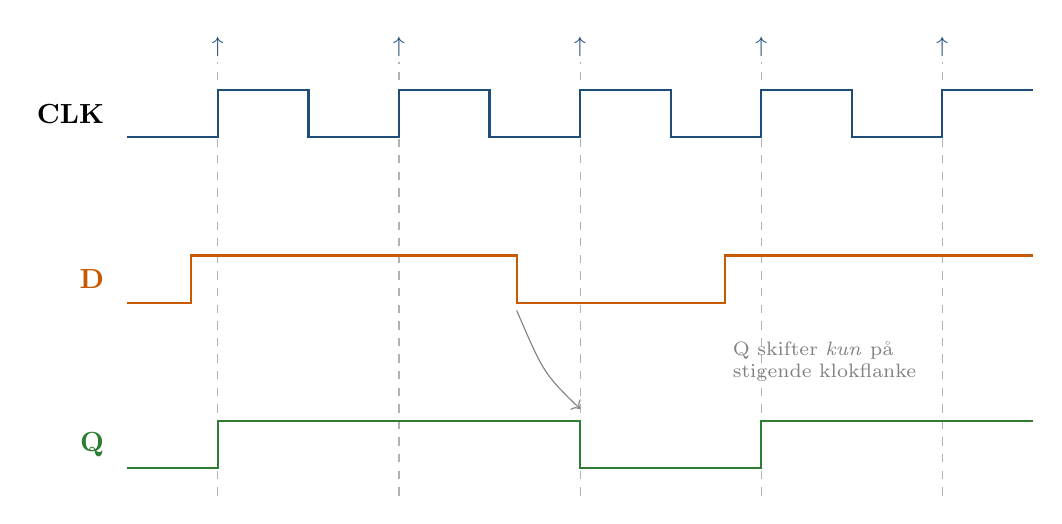
\begin{tikzpicture}[x=1.15cm, y=1cm]
  \def\clky{4.2}\def\dy{2.1}\def\qy{0}\def\h{0.6}

  % labels
  \node[left, font=\bfseries] at (-0.15,\clky+\h/2) {CLK};
  \node[left, font=\bfseries, dcol] at (-0.15,\dy+\h/2) {D};
  \node[left, font=\bfseries, qcol] at (-0.15,\qy+\h/2) {Q};

  % rising-edge sample lines (drawn first, behind signals)
  \foreach \t in {1,3,5,7,9} {
    \draw[dashed, gray!60] (\t,\qy-0.35)--(\t,\clky+\h+0.35);
    \node[accent, font=\footnotesize\bfseries] at (\t,\clky+\h+0.55) {$\uparrow$};
  }

  % CLK
  \draw[thick, accent]
    (0,\clky)--(1,\clky)--(1,\clky+\h)--(2,\clky+\h)--(2,\clky)--(3,\clky)--(3,\clky+\h)--(4,\clky+\h)--(4,\clky)--(5,\clky)--(5,\clky+\h)--(6,\clky+\h)--(6,\clky)--(7,\clky)--(7,\clky+\h)--(8,\clky+\h)--(8,\clky)--(9,\clky)--(9,\clky+\h)--(10,\clky+\h);
  % D  (changes at 0.7, 4.3, 6.6 -- NOT on clock edges)
  \draw[thick, dcol]
    (0,\dy)--(0.7,\dy)--(0.7,\dy+\h)--(4.3,\dy+\h)--(4.3,\dy)--(6.6,\dy)--(6.6,\dy+\h)--(10,\dy+\h);
  % Q  (= D sampled at each rising edge, holds otherwise)
  \draw[thick, qcol]
    (0,\qy)--(1,\qy)--(1,\qy+\h)--(5,\qy+\h)--(5,\qy)--(7,\qy)--(7,\qy+\h)--(10,\qy+\h);

  % annotation: D fell at 4.3 but Q waited until edge at 5
  \draw[->, gray, thin] (4.3,\dy-0.1) .. controls (4.6,1.2) .. (5,\qy+\h+0.15);
  \node[gray, font=\scriptsize, align=left] at (7.7,1.35)
    {Q skifter \emph{kun} på\\stigende klokflanke};
\end{tikzpicture}
\end{document}
